% TODO: add tiling strategy to cope with memory contrains. Mention that it does
% not impact run time.

% TODO: figure out the impact of the important function on the overall runtime.
% Redo the individual tests with real parameters and compare real runtime with
% lab runtimes (individual runtimes added)

% TODO: If individual stuff is really the bottle neck, then analyse how much in
% each layer and compare to cuDNN. Mention that cuDNN is the new standard and
% has outperformed Alex's implementation.

% TODO: Masking and impact of masking for feature learning, manifold learning
% and segmentation. Also lesion prior for segmentation and impact

% \chapter[Accelerating the Training of 3D Convolutional Models by Training in the
% Frequency Domain]{Accelerating the Training of\\ 3D Convolutional Models by\\
% Training in the Frequency Domain}
\chapter{Training of Convolutional Models in the Frequency Domain}
\label{sec:training}

\section[Related work]{Related Work}

Deep learning has traditionally been computationally expensive and advances in
training methods have been the prerequisite for expanding its application to a
variety of image classification problems. The development of layer-wise training
methods \citep{hinton2006b} greatly improved the efficiency of the training of
deep belief networks (DBNs), which has made feasible the use of large sets of
small images (e.g. \num{28x28}), such as those used for hand-written digit
recognition. Subsequently, new directions for speeding up the training of deep
models were opened with the advance of programmable graphics cards (GPUs), which
can perform thousands of operations in parallel. \citet{raina2009} demonstrated
that by using graphics cards, training of restricted Boltzmann machines (RBMs)
on small image patches (e.g. \num{24x24}) can be performed up to \num{70} times
faster than on the CPU, facilitating the application to larger training sets.
However, the number of trainable weights of a DBN increases greatly with the
resolution of the training images, which can make training on large images
impracticable. In order to scale DBNs to high-resolution images,
\citet{lee2009,lee2011} introduced the convolutional deep belief network
(convDBN), a deep generative model that uses weight sharing to reduce the number
of trainable weights. They showed that a convDBN can be used to classify images
with a resolution up to \num{200x200} pixels. To speed up the training of
convolutional neural networks (CNNs) on high-resolution images,
\citet{krizhevsky2012} replaced traditional convolutions of the first layer of
their CNN with strided convolutions, a type of convolution that shifts the
filter kernel as a sliding window with a fixed step size or stride greater than
one. Through the use of strided convolutions, the number of hidden units in each
convolutional layer is greatly reduced, which reduces both training time and
required memory. Using a highly optimized GPU implementation of convolutions,
they were able to train a CNN on images with a resolution of \num{256x256}
pixels, achieving state-of-the-art performance on the ILSVRC-2010 and
ILSVRC-2012 competitions \citep{krizhevsky2012}. An alternative approach for
calculating convolutions was proposed by \citet{mathieu2013} who sped up the
training of CNNs by calculating convolutions between batches of images and
filters using fast Fourier transforms (FFTs), albeit at the cost of additional
memory required for storing the filters. Recently, NVIDIA have released a
library called cuDNN \cite{chetlur2014} that provides GPU-optimized
implementations of 2D and 3D convolutions among other operations that are
frequently used to implement deep learning methods, which further reduces
training times compared to the previous state-of-the-art.

\section{Overview}

In this chapter, we detail our training algorithm and GPU implementation in
full, with a thorough analysis of the running time on high-resolution 2D images
(\num{512x512}) and 3D volumes (\num{128x128x128}), showing speed-ups of up to
8-fold and 200-fold, respectively for training RBMs and a 7-fold speed up for
computing key operations for the training CNNs compared to cuDNN. The proposed
method performs training in the frequency domain, which replaces the calculation
of time-consuming convolutions with simple element-wise multiplications, while
adding only a small number of FFTs. In contrast to similar FFT-based approaches
\citep[e.g.,][]{mathieu2013}, our method does not use batch processing of the
images as a means to reduce the number of FFT calculations, but rather minimizes
FFTs even when processing a single image, which significantly reduces the
required amount of scarce GPU memory.
% We show that our method can be efficiently implemented on multiple graphics
% cards, further improving the runtime performance over other GPU-accelerated
% training methods.
In addition, we formalize the expression of the strided convolutional DBN
(sconvDBN), a type of convDBN that uses strided convolutions to speed up
training and reduce memory requirements, in terms of stride-1 convolutions,
which enables the efficient training of sconvDBNs in the frequency domain.

% TODO: Follow up with how to train them in the medical domain.
% Introduction and motivation. Talks about special challenges. Training in the
% frequency domain is important and a main contribution of this thesis. This will
% be about my algorithm, how it works for convRBMs and CNNs. Especially the tricks
% needed for strided convolutions.

\section{Algorithm}

% Mapping in the frequency domain. Minimize transforms. Also memory
% considerations and the likes. Also trick to do strided convolutions in the
% frequency domain.

\subsection[Training in the spatial domain]{Training in the Spatial Domain}

% Short revision of how training works. Put all the pieces together to make it
% an algorithm. Make sure that I do this for convRBMs

Before we look at the training algorithm of convRBMs in the frequency domain,
let us revise the basic steps for training in the spatial domain. The weights
and bias terms of a convRBM can be learned by CD. During each iteration of the
algorithm, the gradient of each parameter is estimated and a gradient step with
a fixed learning rate is applied. The gradient of the filter weights can be
approximated by
\begin{equation}
\Delta \vect{w}^{(ij)} \approx
\frac{1}{N}(\vect{v}^{(i)}_n*\tilde{\vect{h}}^{(j)}_n -
\vect{v}'^{(i)}_n*\tilde{\vect{h}}_n'^{(j)})
\label{eq:convgra}
\end{equation}
where $\vect{v}_n, n \in [1,N]$ are images from the training set,
$\vect{h}_n^{(j)}$ and $\vect{h}'^{(j)}_n$ are samples drawn from
$p(\vect{h}^{(j)} \given \vect{v}_n)$ and $p(\vect{h}^{(j)} \given
\vect{v}'_n)$, and $\vect{v}'^{(i)}_n = \E[\vect{v}^{(i)} \given \vect{h}_n]$.
To apply the model to real-valued data like certain types of images, the visible
units can be modeled as Gaussian units.
When the visible units are mean--centered and standardized to unit variance, the
expectation of the visible units is given by
\begin{equation} 
\E[\vect{v}^{(i)} \given \vect{h}] = \sum_{j=1}^{N_\text{k}}
\vect{w}^{(ij)}*\vect{h}^{(j)} + b_i
\label{eq:convvis}
\end{equation}
A binary hidden unit can only encode two states. In order to increase the
expressive power of the hidden units, we use noisy rectified linear units as the
hidden units, which have been shown to improve the learning performance
of RBMs \citep{nair2010}. The hidden units can be sampled with
\begin{align} 
\vect{h}^{(j)} &\sim \max(0, \mu^{(j)} + \Norm(0, \sigm(\mu^{(j)}))) \\
\mu^{(j)} &= \sum_{i=1}^{N_\text{c}}\tilde{\vect{w}}^{(ij)}*\vect{v}^{(i)} +c_j
\label{eq:convhid}
\end{align} 
where $\Norm(0, \sigma^2)$ denotes Gaussian noise. The learning algorithm in the
spatial domain is summarized in Figure~\ref{alg:spatial}.

\begin{figure}[t!]
\hspace{-1.75em}
\subfloat[Training in the spatial domain]{
\label{alg:spatial}
\begin{minipage}{0.495\linewidth}
\footnotesize
\begin{algorithm}[H]
\setstretch{1.25}
%\renewcommand{\baselinestretch}{1.25}
%\selectfont
\SetKwInOut{Input}{input}
\SetKwInOut{Output}{output}
\Input{Images $\data = \{\vect{V}_n \given n \in [1, N]\}$}
\Output{Weights gradient $\Delta \vect{w}$}
$\Delta \vect{w} = 0$\;
\ForEach{image $\vect{v} \in \data$} {
  $\vect{v}' = 0$\;
  \For{$j = 1$ \KwTo $N_\text{k}$} {
    $\mu^{(j)} = \sum_{i=1}^{N_\text{c}} \tilde{\vect{w}}^{(ij)} *
    \vect{v}^{(i)} + c_j$\; \mbox{}\\
    \BlankLine
    $\vect{h}^{(j)} \sim \max(0, \mu^{(j)} + \Norm(0, \sigm(\mu^{(j)})))$\;
    \mbox{}\\
    \For{$i = 1$ \KwTo $N_\text{c}$} {
      $\Delta \vect{w}^{(ij)} = \Delta \vect{w}^{(ij)} + \tilde{\vect{h}}^{(j)}
      * \vect{v}^{(i)}$\;
      $\vect{v}'^{(i)} = \vect{v}'^{(i)} + \vect{w}^{(ij)} * \vect{h}^{(j)}$\;
    }
  }
  $\forall i \colon \vect{v}'^{(i)} = \vect{v}'^{(i)} + b_i$\;
  \For{$j = 1$ \KwTo $N_\text{k}$} {
    $\mu'^{(j)} = \sum_{i=1}^{N_\text{c}} \tilde{\vect{w}}^{(ij)} *
    \vect{v}'^{(i)} + c_j$\; \mbox{}\\
    $\vect{h}'^{(j)} \sim \max(0, \mu'^{(j)} +$\\ \hfill $\Norm(0,
    \sigm(\mu^{(j)})))$\; \mbox{}\\
    \For{$i = 1$ \KwTo $N_\text{c}$} {
      $\Delta \vect{w}^{(ij)} = \Delta \vect{w}^{(ij)} - \tilde{\vect{h}}'^{(j)}
      * \vect{v}'^{(i)}$\;
    }
  }
}
\end{algorithm}
\end{minipage}
}
\subfloat[Training in the frequency domain]{
\label{alg:frequency}
\begin{minipage}{0.495\linewidth}
\footnotesize
\begin{algorithm}[H]
\setstretch{1.25}
%\renewcommand{\baselinestretch}{1.25}
%\selectfont
\SetKwInOut{Input}{input}
\SetKwInOut{Output}{output}
\Input{Images $\hat{\data} = \{\hat{\vect{v}}_n \given n \in [1, N]\}$}
\Output{Weights gradient $\Delta\hat{\vect{w}}$}
$\Delta\hat{\vect{w}} = 0$\;
\ForEach{image $\hat{\vect{v}} \in \hat{\data}$} {
  $\hat{\vect{v}}' = 0$\;
  \For{$j = 1$ \KwTo $N_\text{k}$} {
    $\hat{\mu}^{(j)} = \sum_{i=1}^{N_\text{c}} \overline{\hat{\vect{w}}^{(ij)}}
    \cdot \hat{\vect{v}}^{(i)}$\; 
    $\mu^{(j)} = \ifft(\hat{\mu}^{(j)}) + c_j$\;
    $\vect{h}^{(j)} \sim \max(0, \mu^{(j)} + \Norm(0, \sigm(\mu^{(j)})))$\;
    $\hat{\vect{h}}^{(j)} = \fft(\vect{h}^{(j)})$\;
    \For{$i = 1$ \KwTo $N_\text{c}$} {
      $\Delta\hat{\vect{w}}^{(ij)} = \Delta\hat{\vect{w}}^{(ij)} +
      \overline{\hat{\vect{h}}^{(j)}} \cdot \hat{\vect{v}}^{(i)}$\;
      $\hat{\vect{v}}'^{(i)} = \hat{\vect{v}}'^{(i)} + \hat{\vect{w}}^{(ij)}
      \cdot \hat{\vect{h}}^{(j)}$\;
    }
  }
  $\forall i \colon \hat{v}_{0,0}'^{(i)} = \hat{v}_{0,0}'^{(i)} +
  N_\text{v}^2b_i$\;
  \For{$j = 1$ \KwTo $N_\text{k}$} {
    $\hat{\mu}'^{(j)} = \sum_{i=1}^{N_\text{c}} \overline{\hat{\vect{w}}^{(ij)}}
    \cdot \hat{\vect{v}}'^{(i)}$\;
    $\mu'^{(j)} = \ifft(\hat{\mu}'^{(j)}) + c_j$\;
    $\vect{h}'^{(j)} \sim \max(0, \mu'^{(j)} +$ \\
    \hfill $\Norm(0,\sigm(\mu^{(j)})))$\;
    $\hat{\vect{h}}'^{(j)} = \fft(\vect{h}'^{(j)})$\;
    \For{$i = 1$ \KwTo $N_\text{c}$} {
      $\Delta\hat{\vect{w}}^{(ij)} = \Delta\hat{\vect{w}}^{(ij)} -
      \overline{\hat{\vect{h}}'^{(j)}} \cdot \hat{\vect{v}}'^{(i)}$\;
    }
  }
}
\end{algorithm}
\end{minipage}
}
\caption[Comparison of training algorithms of convRBMs in the
spatial and frequency domain]{Comparison of training algorithms of convRBMs in
(a) the spatial and (b) the frequency domain. Training in the frequency domain replaces the $5N_\text{k}N_\text{C}$ convolutions required in the spatial domain with simple
element-wise multiplications, while adding only $4N_\text{k}$ Fourier
transforms. The other operations are equivalent in both domains.}
\label{fig:algorithms}
\end{figure}

\subsection[Training in the frequency domain]{Training in the Frequency Domain}

The computational bottleneck of the training algorithm in the spatial domain is
the calculation of convolutions, which needs to be performed $5 \times
N_\text{c} \times N_\text{k}$ times per iteration. To speed up the calculation
of convolutions, we perform training in the frequency domain, which maps the
convolutions to simple element-wise multiplications. This is especially
important for the training on 3D images due to the relatively large number of
weights of a 3D kernel compared to 2D. To minimize the number of Fourier
transforms, we map all operations needed for training to the frequency domain
whenever possible, which allows the training algorithm to stay almost entirely
in the frequency domain. All of the scalar operations needed for training
(multiplications and additions) can be readily mapped to the frequency domain
because the Fourier transform is a linear operation. Another necessary operation
is the flipping of a convolutional kernel, $\tilde{w}(u,v) =
w(N_\text{w}-u+1,N_\text{w}-v+1)$. To calculate flipping efficiently, we reindex
the weights of a convolutional kernel $w^{(ij)}_{uv}$ from $u,v \in [1,
N_\text{w}]$ to $u,v \in [-\lfloor
N_\text{w}/2\rfloor,\lfloor(N_\text{w}-1)/2\rfloor$, which simplifies the
calculation of a flipped kernel to $\tilde{w}(u,v) = w(-u,-v)$.
This allows flipping of a kernel in the spatial domain to be expressed by the
element-wise calculation of the complex conjugate in the frequency domain, which
follows directly from the time-reversal property of the Fourier transform, if
$h(x) = f(-x)$, then $\hat{h}(\xi) = \hat{f}(-\xi)$; and the reality condition,
$\hat{f}(-\xi)=\overline{\hat{f}(\xi)}$, where $\hat{x} = \F(x)$ denotes
$x$ in the frequency domain. Using the aforementioned mappings, equations
\ref{eq:convgra} to \ref{eq:convhid} can be rewritten as
\begin{align}
\Delta \hat{\vect{w}}^{(ij)} &=
\hat{\vect{v}}^{(i)}\cdot\overline{\hat{\vect{h}}^{(j)}} - \hat{\vect{v}}'^{(i)}
\cdot \overline{\hat{\vect{h}}'^j} \\
\E[\hat{v}_{xy}^{(i)} \given \vect{\hat{h}}] &=
\begin{dcases}
\sum_{j=1}^{N_\text{k}}\hat{w}_{xy}^{(ij)}\hat{h}_{xy}^{(j)} + N_\text{v}^2
b_i & \text{for } x,y = 0 \\
\sum_{j=1}^{N_\text{k}}\hat{w}_{xy}^{(ij)}\hat{h}_{xy}^{(j)} & \text{for } x,y
\neq 0 \end{dcases} \\
\hat{\vect{h}}^{(j)} &\sim \F\left(\max(0, \F^{-1}(\hat{\mu}^{(j)}) + c_j + 
\Norm(0, \sigma^2))\right) \\
\hat{\mu}^j
&=\sum_{i=1}^{N_\text{c}}\overline{\hat{\vect{w}}^{(ij)}}\cdot\hat{\vect{v}}^{(i)}
\end{align}
where $\sigma^2 = \sigm(\F^{-1}(\hat{\mu}^{(j)})+c_j)$, $\F^{-1}$ denotes the
inverse Fourier transform, and $\cdot$ denotes element-wise multiplication. The
algorithm for approximating the gradient in the frequency domain is summarized
in Figure~\ref{alg:frequency}.

The only operations that cannot be directly mapped to the frequency domain are
the calculation of the maximum function, the generation of Gaussian noise, and
trimming of the filter kernels. To perform the first two operations, an image
needs to be mapped to the spatial domain and back. However, these operations
need only be calculated $2N_\text{k}$ times per iteration and are therefore not
a significant contributor to the total running time. Because filter kernels are
padded to the input image size, the size of the learned filter kernels must be
explicitly enforced by trimming. This is done by transferring the filter kernels
to the spatial domain, setting the values outside of the specified filter kernel
size to zero, and then transforming the filter kernels back to the frequency
domain. This procedure needs to be performed only once per mini-batch. Since the
number of mini-batches is relatively small compared to the number of training
images, trimming of the filter kernels also does not add significantly to the
total running time of the training algorithm. Although we have presented the
algorithm in the context of training convRBMs, the same mapping of operations
can be used to speed up the training of other convolutional models, such as
convolutional neural networks.

\subsection[Mapping of strided convolutions to stride-1 convolutions]{Mapping of
Strided Convolutions to Stride-1 Convolutions}
\label{sec:training:strided}

% Strided convolutions are a type of convolution that shifts the filter kernel as
% a sliding window with a step size or stride $s > 1$, stopping at only $N_\text{v}
% / s$ positions. This reduces the number of hidden units per channel to
% $N_\text{h} = N_\text{v} / s$, hence significantly reducing training times and
% memory required for storing the hidden units during training. The energy of a
% strided convolutional RBM (sconvRBM) is defined as
% \begin{equation}
% E(\vect{v},\vect{h}) =
% -\sum_{i=0}^{N_\text{c}-1}\sum_{j=0}^{N_\text{k}-1}\sum_{x,y=0}^{N_\text{h}-1}
% \sum_{u,v=-\lfloor N_\text{w}/2\rfloor}^{\lfloor(N_\text{w}-1)/2\rfloor}
% \hspace{-1.2em}h_{xy}^jw_{uv}^{ij}v_{sx+u, sy + v}^i -
% \sum_{i=0}^{N_\text{c}-1}b_i\!\sum_{x,y = 0}^{N_\text{v}-1}\!v_{xy}^i -
% \sum_{j=0}^{N_\text{k}-1}c_j\!\sum_{x,y = 0}^{N_\text{h}-1}\!h_{xy}^j
% \end{equation}

Convolutions with a stride $s > 1$ can be expressed equivalently as convolutions
with stride $s = 1$ by reorganizing the values of $\vect{v}^{(i)}$ and
$\vect{w}^{(ij)}$ to $\vect{V}^{(i')}$ and $\vect{W}^{(i'j)}$ as illustrated in
\ref{fig:npcDBN}. This reindexing scheme allows the energy function to be
expressed in terms of conventional (stride-1) convolutions, which facilitates
training in the frequency domain. The new indices of $V^{(i')}_{x'y'}$ and
$W^{(i'j)}_{u'v'}$ can be calculated from the old indices of $v^i_{(xy)}$ and
$w^{(ij)}_{uv}$ as follows:
\begin{align}
x' &= \lfloor (x-1) / s \rfloor + 1 & u' &= \lfloor (u-1) / s \rfloor + 1 \\
y' &= \lfloor (y-1) / s \rfloor + 1 & v' &= \lfloor (v-1) / s \rfloor + 1\\
i' &= s^2(i-1) + s((y-1) \bmod{s}) + ((x-1) \bmod{s}) + 1
\end{align}

\begin{figure}[tb]
\centering
\begin{tikzpicture}[node distance=0.9cm and 4.5cm]

\tikzstyle{every node}+=[font=\scriptsize\sffamily]
\tikzstyle{label}=[font=\footnotesize\sffamily]
\tikzstyle{lines}=[dashed,opacity=0]
\tikzstyle{mymatrix}=[%
  matrix of nodes,%
  inner sep=0pt,
  nodes={inner sep=2pt},
  %draw,%
  left delimiter  = (,%
  right delimiter = )%
]

\tikzstyle{every pin}+=[inner sep=2pt,align=center,pin
distance=0.1cm,font=\footnotesize\sffamily]

% \matrix [mymatrix] (image) {
% |[red]|4  & |[green]|5  & |[red]|1  & |[green]|2  & |[red]|1  & |[green]|2  \\
% |[blue]|4 & |[yellow]|2 & |[blue]|5 & |[yellow]|1 & |[blue]|1 & |[yellow]|2 \\
% |[red]|4  & |[green]|5  & |[red]|1  & |[green]|2  & |[red]|1  & |[green]|2  \\
% |[blue]|4 & |[yellow]|2 & |[blue]|5 & |[yellow]|1 & |[blue]|1 & |[yellow]|2 \\
% |[red]|4  & |[green]|5  & |[red]|1  & |[green]|2  & |[red]|1  & |[green]|2  \\
% |[blue]|4 & |[yellow]|2 & |[blue]|5 & |[yellow]|1 & |[blue]|1 & |[yellow]|2 \\
% };

\matrix [mymatrix] (image) {
4 & 2 & 1 & 8 & 2 & 7 \\
4 & 2 & 3 & 4 & 3 & 1 \\
3 & 4 & 5 & 5 & 1 & 2 \\
7 & 5 & 1 & 2 & 2 & 3 \\
2 & 1 & 2 & 2 & 7 & 5 \\
6 & 9 & 5 & 4 & 6 & 6 \\
};

\matrix [mymatrix, below=of image] (kernel) {
0.1 & -0.1 & 0.3 & 0.4 \\
0.2 & -0.3 & 0.1 & 0.1 \\
-0.4 & 0.2 & 0.2 & -0.3 \\
0.5 & -0.2 & -0.2 & 0.4 \\
};

\matrix [mymatrix, below=of kernel,thick] (map) {
%\matrix [mymatrix, above=of image,thick] (map) {
|[red]|\bfseries 6.8 & |[blue]|\bfseries 2  \\
\bfseries 4.6 &  \bfseries 3.6 \\
};

\node[fit=(image-1-1)(image-4-4), xshift=-0.5pt, yshift=-0.5pt, draw=red,inner
sep=0,thick] (window1) {};

\node[fit=(image-1-3)(image-4-6), xshift=0.5pt, yshift=0.5pt, draw=blue,inner
sep=0,thick,pin=45:{Sliding filter\\ window}] (window2) {};

\draw[decorate,decoration={brace,raise=1pt}] (window1.north
west|-window2.north west)--node[above=3pt,fill=white,fill opacity=0.5,text
opacity=1,font=\small]{$s$}(window2.north west);

\begin{pgfonlayer}{background}
\foreach \x in {1,3,5} {
  \foreach \y in {1,3,5}
    \node[fit=(image-\x-\y),inner sep=0, fill=red!15] {};
  \foreach \y in {2,4,6}
    \node[fit=(image-\x-\y),inner sep=0, fill=green!15] {};
}
\foreach \x in {2,4,6} {
  \foreach \y in {1,3,5}
    \node[fit=(image-\x-\y),inner sep=0, fill=blue!15] {};
  \foreach \y in {2,4,6}
    \node[fit=(image-\x-\y),inner sep=0, fill=yellow!30] {};
}
\foreach \x in {1,3} {
  \foreach \y in {1,3}
    \node[fit=(kernel-\x-\y),inner sep=0, fill=red!15] {};
  \foreach \y in {2,4}
    \node[fit=(kernel-\x-\y),inner sep=0, fill=green!15] {};
}
\foreach \x in {2,4} {
  \foreach \y in {1,3}
    \node[fit=(kernel-\x-\y),inner sep=0, fill=blue!15] {};
  \foreach \y in {2,4}
    \node[fit=(kernel-\x-\y),inner sep=0, fill=yellow!30] {};
}
\end{pgfonlayer}

\node[align=center] at ($(image.south)!0.5!(kernel.north)$) {\footnotesize $*$\\
(with a step size of $s$)};

%\node at ($(image.north)!0.5!(map.south)$) {$=$};
\node[label] at ($(kernel)!0.65!(map)$) {$=$};

\begin{scope}[on grid,node distance=2cm and 1.95cm] 
\matrix [mymatrix, right=3.8cm of image,fill=red!15] (image1) {
4 & 1 & 2 \\
3 & 5 & 1 \\
2 & 2 & 7 \\
};

\matrix [mymatrix, right=of image1,fill=green!15] (image2) {
2 & 8 & 7 \\
4 & 5 & 2 \\
1 & 2 & 5 \\
};

\matrix [mymatrix, right=of image2,fill=blue!15] (image3) {
4 & 3 & 3 \\
7 & 1 & 2 \\
6 & 5 & 6 \\
};

\matrix [mymatrix, right=of image3,fill=yellow!30] (image4) {
2 & 4 & 1 \\
5 & 2 & 3 \\
9 & 4 & 6 \\
};

\matrix [mymatrix, right=3.8cm of kernel,fill=red!15] (kernel1) {
0.1 & 0.3 \\
-0.4 & 0.2 \\
};

\matrix [mymatrix, right=of kernel1,fill=green!15] (kernel2) {
-0.1 & 0.4 \\
0.2 & -0.3 \\
};

\matrix [mymatrix, right=of kernel2,fill=blue!15] (kernel3) {
0.2 & 0.1 \\
0.5 & -0.2 \\
};

\matrix [mymatrix, right=of kernel3,fill=yellow!30] (kernel4) {
-0.3 & 0.1 \\
-0.2 & 0.4 \\
};

\matrix [mymatrix, right=3.8cm of map] (map1) {
\textcolor{red}{0.5} & \textcolor{blue}{-1.1}  \\
1.4 & 1.4 \\
};
\matrix [mymatrix, right=of map1] (map2) {
\textcolor{red}{2.3} & \textcolor{blue}{2.4}  \\
1.2 & -0.8   \\
};
\matrix [mymatrix, right=of map2] (map3) {
\textcolor{red}{4.4} & \textcolor{blue}{1}  \\
3.5 & 1.7  \\
};
\matrix [mymatrix, right=of map3] (map4) {
\textcolor{red}{-0.4} & \textcolor{blue}{-0.3}  \\
-1.5 & 1.3 \\
};
\matrix [mymatrix, right=of map4, thick] (map5) {
|[red]|\textbf{6.8} & |[blue]|\textbf{2}  \\
\textbf{4.6} & \textbf{3.6}   \\
};

\foreach \x in {1,...,4} {
  \node[fit=(image\x-1-1)(image\x-2-2), draw=red,inner sep=0,thick,
  xshift=-0.5pt, yshift=-0.5pt] {};
  
  \node[fit=(image\x-1-2)(image\x-2-3), draw=blue,inner sep=0,thick,
  xshift=0.5pt, yshift=0.5pt] {};
  \node[label] at ($(image\x.south)!0.5!(kernel\x.north)$) {$*$};
  %\node at ($(image\x.north)!0.5!(map\x.south)$) {$=$};
  \node[label] at ($(kernel\x)!0.65!(map\x)$) {$=$};
}

\node at ($(map1.east)!0.5!(map2.west)$) {$+$};
\node at ($(map2.east)!0.5!(map3.west)$) {$+$};
\node at ($(map3.east)!0.5!(map4.west)$) {$+$};
\node at ($(map4.east)!0.5!(map5.west)$) {$=$};

\node[left=1.85cm of image,rotate=90,label] {Image $\vect{v}^{(1)}$};
\node[left=1.85cm of kernel,rotate=90,align=center,label]
{Filter $\vect{w}^{(1,j)}$};
\node[left=1.85cm of map,rotate=90,align=center,label] (maplabel)
{Feature};
\node[right=1em of maplabel,rotate=90,label] {map $\vect{h}^{(j)}$};

\draw[->,shorten <=10pt, shorten >=10pt] (image)--
node[above,label]{Rearrange}node[below,label]{pixels}(image1);

\draw[->,shorten <=10pt, shorten >=10pt] (kernel)--
node[above,label]{Rearrange}node[below,label]{pixels}(kernel1);

\foreach\x in {1,...,4} {
\draw[decorate,decoration={brace,raise=2pt}]
(image\x.south east)--node[below=4pt,label]
{$\vect{V}^{(\x)}$} (image\x.south west);

\draw[decorate,decoration={brace,raise=2pt}]
(kernel\x.south east)--node[below=4pt,label]
{$\vect{W}^{(\x,j)}$} (kernel\x.south west);
}

\draw[decorate,decoration={brace,raise=2pt}]
(map5.south east)--node[below=4pt,label]
{$\vect{h}^{(j)}$} (map5.south west);

\end{scope}

\end{tikzpicture}

\caption[Mapping of strided convolutions to stride-1 convolutional]{Illustration
of convolutions with a sliding window step size $s = 2$ as used during filtering in a sconvDBN. A convolution of a given stride size (left
side) can be efficiently calculated as the sum of multiple individual
convolutions with $s = 1$ (right side) after rearranging the pixels of the input
image and the filter kernels. The bottom row shows the actual values produced by
the convolutions, which are the features from the image extracted by the filter.
The figure is best viewed in color.}
\label{fig:npcDBN}
\end{figure}

After reorganizing $\vect{v}^{(i)}$ and $\vect{w}^{(ij)}$ to $\vect{V}^{(i')}$
and $\vect{W}^{(i'j)}$, the energy of the model can be rewritten as
\begin{align} 
E(\vect{V},\vect{h}) &= 
-\sum_{i=1}^{N_\text{C}}\sum_{j=1}^{N_\text{k}}\sum_{x,y=1}^{N_\text{h}}
\sum_{u,v=1}^{N_\text{W}}
h_{xy}^{(j)}W_{uv}^{(ij)}V_{x+u-1, y+v-1}^{(i)}
- \sum_{i=1}^{N_\text{C}}b_i\!\sum_{x,y = 1}^{N_\text{V}}\!V_{xy}^{(i)}
- \sum_{j=1}^{N_\text{k}}c_j\!\sum_{x,y = 1}^{N_\text{h}}\!h_{xy}^{(j)}\\
&= -\sum_{i=1}^{N_\text{C}} \sum_{j=1}^{N_\text{k}}
\vect{h}^{(j)}\bullet (\tilde{\vect{W}}^{(ij)} * \vect{V}^{(i)}) -
\sum_{i=1}^{N_\text{C}}b_i\!\sum_{x,y = 1}^{N_\text{V}}\!V_{xy}^{(i)} -
\sum_{j=1}^{N_\text{k}}c_j\!\sum_{x,y = 1}^{N_\text{h}}\!h_{xy}^{(j)}
\end{align}
where $*$ denotes periodic convolution. The number of channels, number of
visible units per channel and number of weights per channel after reorganization
are given by $N_\text{C} = N_\text{c} \times s^2$, $N_\text{V}^2 = N_\text{v}^2
/ s^2$ and $N_\text{W}^2 = N_\text{w}^2 / s^2$, respectively.

\subsection[GPU implementation and memory considerations]{GPU Implementation and
Memory Considerations}

To further reduce training times, the algorithm can be efficiently implemented
on graphics cards, which can perform hundreds of operations in parallel.
To optimize efficiency, it is crucial to maximize the utilization of the large
number of available GPU cores, while minimizing the required amount of GPU
memory. Because our algorithm requires only a relatively small number of FFT
calculations per iteration, the computational bottleneck is the calculation of
the element-wise operations, which can be performed in parallel. Thus we
distribute the processing of a single 2D image over $N_\text{v}(\lfloor
N_\text{v}/2 \rfloor + 1) \times N_\text{c}$ independent threads, with one
thread per element in the frequency domain. The large number of parallel threads
results in a high utilization of the GPU, even when each image of a mini-batch
is processed sequentially, which we do in our method because this greatly
reduces the amount of GPU memory required to store the visible and hidden units
compared to processing batches of images in parallel.

Due to the relatively small amount of GPU memory compared to CPU memory, memory
requirements are an important consideration when designing a GPU algorithm.
However, the total amount of required memory is highly implementation-dependent
(e.g. the use of temporary variables for storing intermediate results) and a
comparison can only be done with common elements at the algorithmic level.
Therefore, in the remainder of this section, we focus on the memory requirements
of key variables such as the visible units, the hidden units, and the filters,
which are required by all implementations. In our training algorithm, all key
variables are stored in the frequency domain, where each element in the
frequency domain is represented by a single-precision complex number. Due to the
symmetry of the Fourier space, the number of elements that need to be stored is
roughly half the number of elements in the spatial domain. Thus, the memory
required for storing the visible and hidden units in the frequency domain is
roughly the same as in the spatial domain. A potential drawback of training in
the frequency domain is that the filters need to be padded to the size of the
visible units before applying the Fourier transformation, which increases the
memory required for storing the filters on the GPU. The total amount of memory
in bytes required for storing the visible units, hidden units, and padded
filters is given by the sum of their respective terms
\begin{equation} 
% \text{memory}_{\text{freq}} &= 8N_\text{v}(\lfloor N_\text{v}/2 \rfloor +1)
% \times (N_\text{c} + N_\text{k} + N_\text{k}N_\text{c}) \\
% &\approx 4N_\text{v}^2 \times (N_\text{c} + N_\text{k} + N_\text{k}N_\text{c})
% \\
% &\approx
4N_\text{v}^2N_\text{c} + \frac{4N_\text{v}^2 N_\text{k}}{s^2} +
4N_\text{v}^2N_\text{k}N_\text{c}.
\end{equation}
As a comparison, the training method of \cite{krizhevsky2012} processes batches
of images in order to fully utilize the GPU, which requires the storing of
batches of visible and hidden units. The memory needed for storing the key
variables is given by
\begin{equation} 
%\text{memory}_{\text{spat}}= 4N_\text{v}^2 \times (N_\text{b}N_\text{c} +
% N_\text{b}N_\text{k}) + 4N_\text{w}^2N_\text{k}N_\text{c}
4N_\text{v}^2 N_\text{b}N_\text{c} + \frac{4N_\text{v}^2
N_\text{b}N_\text{k}}{s^2} + 4N_\text{w}^2N_\text{k}N_\text{c},
\end{equation}
where $N_\text{b}$ is the number of images per mini-batch. Depending on the
choice of the batch size, this method requires more memory for storing the
visible and hidden units, while requiring less memory for storing the filters.
Alternatively, \citet{mathieu2013} proposed to speed up the training of CNNs by
calculating convolutions between batches of images and filters using FFTs. The
memory required for storing the visible units, hidden units, and filters using
this method is given by
\begin{equation}
%\text{memory}_{\text{freq}} &= 8 N_\text{v}(\lfloor N_\text{v}/2 \rfloor +1)
%\times (N_\text{b}N_\text{c} + N_\text{b}N_\text{k} + N_\text{k}N_\text{c}) \\
%&\approx 
4 N_\text{v}^2 N_\text{b}N_\text{c} + 4
N_\text{v}^2 N_\text{b}N_\text{k} + 4 N_\text{v}^2 N_\text{k}N_\text{c}
\end{equation}
\Ref{tab:memory} shows a comparison of the memory per GPU required for
storing key variables when training a network used in previous work by
\citet{krizhevsky2012}. For the first layer, a comparison with Mathieu et al.'s
training method could not be performed, because that method does not support
strided convolutions, which would significantly reduce the memory required for
storing the hidden units. In all layers, the proposed approach compensates for
the increased memory requirements for the filters by considering one image at a
time rather than a batch, and still outperforms batched learning in the spatial
domain in terms of speed (see \ref{sec:training:eval}), despite not using
batches.

% In all layers, the additional memory required for
% storing the padded filters is smaller than the memory required for storing
% batches of visible and hidden units. Thus, our method requires less memory for
% storing the key variables during training than two state-of-the-art
% GPU-accelerated methods.

\begin{table}[tb]

\caption[Comparison of the memory required for storing key variables using
different training methods]{Comparison of the memory required for storing key
variables using different training methods: our method (Freq), Krizhevsky et
al.'s spatial domain method (Spat), and Mathieu et al.'s method using batched
FFTs (B-FFT). A comparison with Mathieu et al.'s method could not be made for
the first layer, because that method does not support strided convolutions. In
all layers, our method consumes less memory for storing the key variables than
the other two methods.}

\label{tab:memory}
\centering
\sisetup{
  round-mode = places,
  round-precision = 1,
  exponent-product = \cdot,
  detect-weight=true,
  detect-inline-weight=math,
  tight-spacing = false,
  table-align-text-post = false
}%
\begin{tabular}{l
S[table-format=3.0]
S[table-format=3.0]
S[table-format=3.0]
S[table-format=2.0]
S[table-format=3.0]
S[table-format=1.0]
S[table-format=2.1]
S[table-format=3.1]
S[table-format=3.1]}
\toprule
Layer & {$N_\text{b}$} & {$N_\text{v}$} & {$N_\text{c}$} & {$N_\text{w}$} &
{$N_\text{k}$} & {$s$} & \multicolumn{3}{c}{Memory in MB} \\
& & & & & & & {Freq} & {Spat} & {B-FFT}
%{Out Method} & {\citet{Krizhevsky2012}} & {\cite{Mathieu2013}}
\\
\midrule
%1 (without striding) & 128 & 224 & 3 & 11 & 48 & 4 & 37.32422 & 1249.566 &
%1277.062 \\
1 & 128 & 224 & 3 & 11 & 48 & 4 & 28.71094 & 147.0665 & {---} \\
2 & 128 & 55 & 48 & 5 & 128 & 1 & 72.92938 & 260.5469 & 330.8594 \\
3 & 128 & 27 & 128 & 3 & 192 & 1 & 69.23364 & 114.75 & 182.25 \\
4 & 128 & 13 & 192 & 3 & 192 & 1 & 24.01318 & 32.95312 & 55.45312 \\
5 & 128 & 13 & 192 & 3 & 128 & 1 & 16.05005 & 27.25 & 42.25 \\
%\addlinespace
%Total & & & & & & & 210.9372 & 582.5665 & 330.8594 \\
\bottomrule
\end{tabular}\\[0.2em]
\end{table}

\section[Evaluation of running time]{Evaluation of Running Time}
\label{sec:training:eval}

\subsection[Comparison of running times for training sconvDBNs]{Comparison of
Running Times for Training sconvDBNs}

To demonstrate where the performance gains are produced, we trained a two-layer
sconvDBN on 2D and 3D images using our frequency-domain method and the following
methods that all compute convolutions on the GPU, but using different
approaches: 1) our spatial domain implementation that convolves a single 2D or
3D image with a single 2D or 3D filter kernel at a time, 2)~Krizhevsky's spatial
domain convolution implementation \citep{Krizhevsky2012b}, which is a widely
used method \citep[e.g.,][]{scherer2010,hinton2012,zeiler2013} that calculates
the convolution of batches of 2D images and 2D filter kernels in parallel (note
that this method cannot be applied to 3D images, so it was only used for the 2D
experiments), and 3) our implementation that calculates convolutions using FFTs,
but without mapping the other operations that would allow the algorithm to stay
in the frequency domain when not computing convolutions. The parameters that we
used for training convRBMs on 2D and 3D images are summarized in
\ref{tab:parameters}. The key parameters that we varied for our experiments are
the filter size and stride size of the first layer, and the filter size and the
number of channels of the second layer. Because the number of channels of the
second layer is equal to the number of filters of the first layer, we also
varied the number of filters of the first layer in order to attain the desired
number of channels. For all implementations, the training time is directly
proportional to the number of filters. Therefore, a detailed comparison of all
four methods with a varying number of filters was not performed. The hardware
details of our test environment are summarized in \ref{tab:hardware1}.

\begin{table}
\centering
\caption{Training parameters.}
\begin{tabular}{lcccc}
\toprule
Parameter & \multicolumn{2}{c}{ImageNet (2D)} & \multicolumn{2}{c}{OASIS (3D)}
\\
\addlinespace
 & \multicolumn{1}{c}{1st layer} & \multicolumn{1}{c}{2nd layer} 
 & \multicolumn{1}{c}{1st layer} & \multicolumn{1}{c}{2nd layer} \\
\cmidrule(r){1-1} \cmidrule(lr){2-2} \cmidrule(lr){3-3} \cmidrule(lr){4-4}
\cmidrule(l){5-5}
Filter size & 5 to 52 & 5 to 13 & 3 to 36 & 3 to 9 \\
Stride size & 1, 2, 4 & 1 & 1, 2, 4 & 1 \\
Number of channels & 3 & 16, 32, 64 & 1 & 8, 16, 32 \\
Number of filters & 32 & 32 & 32 & 16 \\
Image dimension & $512^2$ & $128^2$ & $128^3$ & $64^3$ \\
Number of images & 256 & 256 & 100 & 100 \\
Batch size & 128 & 128 & 25 & 25 \\
\bottomrule
\end{tabular}
\label{tab:parameters}
\end{table}

\begin{table} 
\centering
\caption{Hardware specification of our test system for training sconvDBNs using
different implementations for calculating convolutions.}
\label{tab:hardware1}
\begin{tabular} {ll}
\toprule
Processor & Intel i7-3770 CPU @ 3.40\,GHz \\
CPU Memory & 8\,GB \\
\addlinespace
Graphics Card & NVIDIA GeForce GTX 660 \\
GPU Cores & 960 cores @ 1.03\,GHz \\
GPU Memory & 2\,GB \\
\bottomrule
\end{tabular}
\end{table}

For the comparison on 2D images, we used a dataset of 256 natural color images
from the ImageNet dataset \citep{deng2009}. All images were resampled to a
resolution of \num{512x512} pixels per color channel. For the evaluation on 3D
images, we used 100 magnetic resonance images (MRIs) of the brain from the OASIS
dataset \citep{marcus2007}. We resampled all volumes to a resolution of
\num{128x128x128} voxels and a voxel size of \SI{2x2x2}{\milli\metre}.

\subsubsection[Running time analysis on 2D color images (ImageNet)]{Running Time
Analysis on 2D Color Images (ImageNet)}

\ref{fig:run_imgnet}\subref{fig:run_imgnet_l1} shows a comparison of running
times for training the first sconvRBM layer on 256 images with varying filter
and stride sizes. Due to internal limitations of Krizhevsky's convolution
implementation, it cannot be applied to images with a resolution of
\num{512x512} pixels when using a stride size smaller than four, and those
comparisons could not be made. Our frequency domain implementation is between 2
to 24 times faster than our convolution implementation, where the speed gains
are larger for larger filter and stride sizes. For a stride of one, the impact
of the convolution implementation on the total running time is relatively low,
because the computational bottleneck is the inference and sampling of the hidden
units.
% For a stride of one, the proportion of the time spend to calculate
% convolutions is small compared to calculating the expectation of the hidden
% units and to sample the hidden units, which reduces the impact of the choice
% of the convolution implementation on the total running time.
% For a stride of one, the running time mostly depends on the time spent to
% calculate the expectation of the hidden units and to sample the hidden units.
As the number of hidden units decreases with larger strides, the running time
becomes more dependent on the time spent to calculate convolutions.
Hence, the differences between the four methods are more pronounced for larger
strides. For a stride of four, training in the frequency domain is between 8 to
24 times faster than training in the spatial domain using our convolution
implementation and 2 to 7 times faster than using batched convolutions.
Calculating convolutions by FFTs is the slowest method for all stride sizes and
2D filter sizes up to 44, largely due to the cost of calculating Fourier
transforms.

\begin{figure}[t!]
\subfloat[Running times of training a first layer sconvRBM
with stride sizes of 1, 2, and 4.] {
\label{fig:run_imgnet_l1}
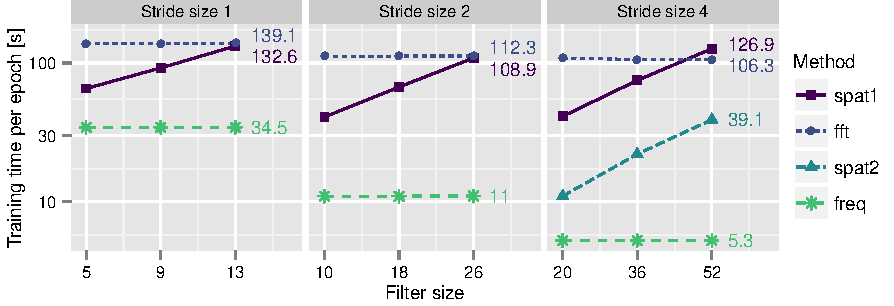
\includegraphics{figures/runtime_imgnet_c3}
%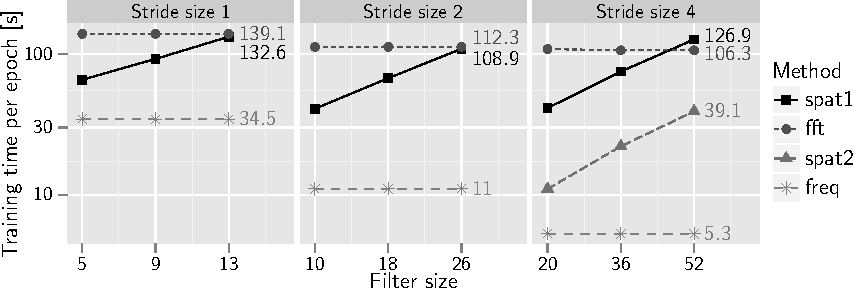
\includegraphics{figures/NECO-03-14-2099-Figure-2}
%\input{r_figures/runtime_imgnet_c3_bw}
}

\subfloat[Running times of training a second layer sconvRBM with
16, 32, and 64 channels (stride size 1).] {
\label{fig:run_imgnet_l2}
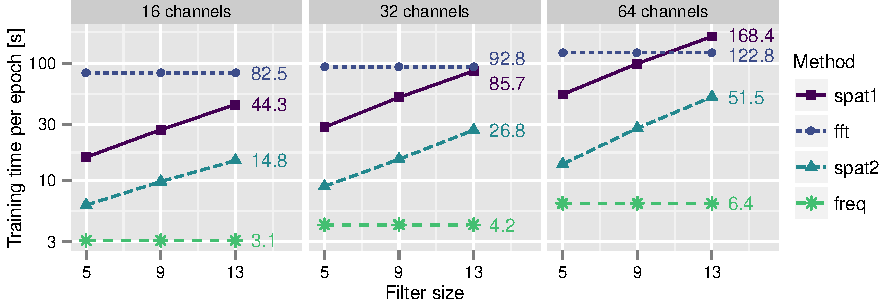
\includegraphics{figures/runtime_imgnet_c16-64}
%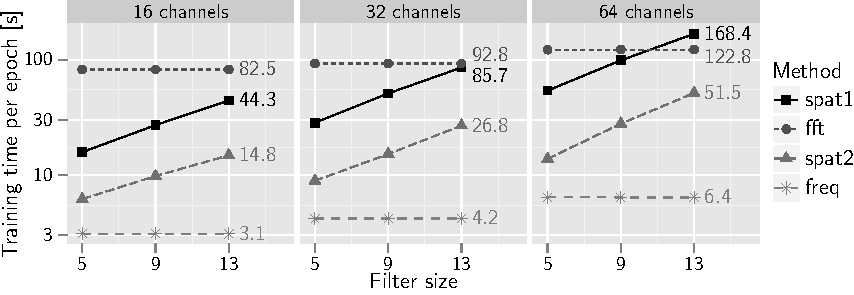
\includegraphics{figures/NECO-03-14-2099-Figure-3}
%\input{r_figures/runtime_imgnet_c16-64_bw}
}

\caption[Comparison of running times for training a sconvRBMs on 2D
images]{Comparison of running times for training a (a) first and (b) second
layer sconvRBM on 2D images using our frequency domain method (freq) and three
alternative methods using different convolution implementations: single image
convolutions (spat1), batched convolutions (spat2), and convolution by using
FFTs (fft). Due to internal limitations of the implementation of batched
convolutions, a comparison with spat2 could not be performed for images with a
resolution of \num{512x512} when using a stride size smaller than four.}
\label{fig:run_imgnet}
\end{figure}

\ref{fig:run_imgnet}\subref{fig:run_imgnet_l2} shows a similar comparison for
training the second convRBM layer for a stride size of one and varying filter
sizes and numbers of channels. In contrast to training the first layer, training
times mostly depend on the calculation of convolutions, where the impact of
calculating convolutions on the total running time increases with an increasing
number of channels. Training in the frequency domain is between 5 to 26 times
faster than training in the spatial domain using single-image convolutions, and
2 to 8 times faster than using batched convolutions. For all channel sizes,
batched training is about 3 to 4 times faster than non-batched training and
calculating convolutions using FFTs is much slower than batched training and
training in the frequency domain. To summarize, training of 2D images in the
frequency domain is much faster than training in the spatial domain even for
small filter sizes. Using the largest filter kernels in both layers, the
proposed method is shown to yield a speedup of 7 to 8 times compared to
state-of-the-art GPU implementations.

\subsubsection{Running Time Analysis on 3D Volumes (OASIS)}

\ref{fig:run_oasis} shows the comparison of running times for training a first
and second layer sconvRBM on 3D volumes for varying filter sizes, stride sizes,
and varying numbers of channels. In contrast to training on 2D images, the
computational costs of calculating 3D convolutions break even with calculating
FFTs even for small filter sizes, because the number of multiplications and
additions per convolution increases cubically, instead of quadratically, with
the filter kernel size. As a result, simply training by convolutions in the
frequency domain is faster than in the spatial domain. However, our proposed
training algorithm still outperforms both other methods, even at the smallest
filter size. For filter sizes of five and larger, our frequency domain
implementation is between 3.5 to 200 times faster than our spatial domain
implementation using single-image convolutions and 2.7 to 17 times faster than
calculating convolutions by FFTs. Similar to the results on 2D images, training
times of the first layer using a stride of one depend strongly on the time
required to calculate the expectation of the hidden units and to sample the
hidden units. Hence, performance improvements of our frequency domain method are
more pronounced for larger strides and numbers of channels, where the impact of
calculating convolutions on the total training time is also larger. This makes
the proposed method particularly suitable for training sconvRBMs on
high-resolution 3D volumes.

\begin{figure}[t!]
\subfloat[Running times of training a first layer sconvRBM with stride sizes of 1, 2, and 4.] {
\label{fig:run_oasis_l1}
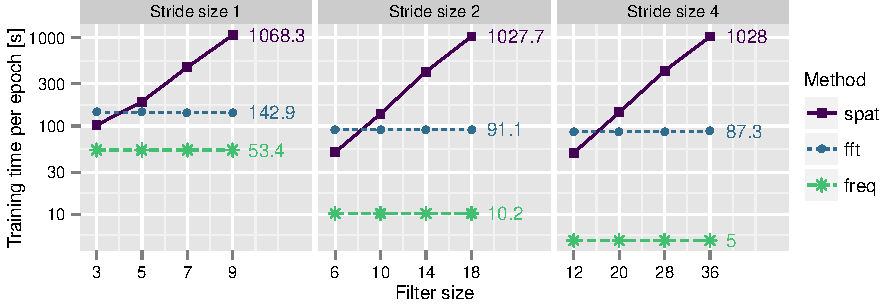
\includegraphics{figures/runtime_oasis_c1}
%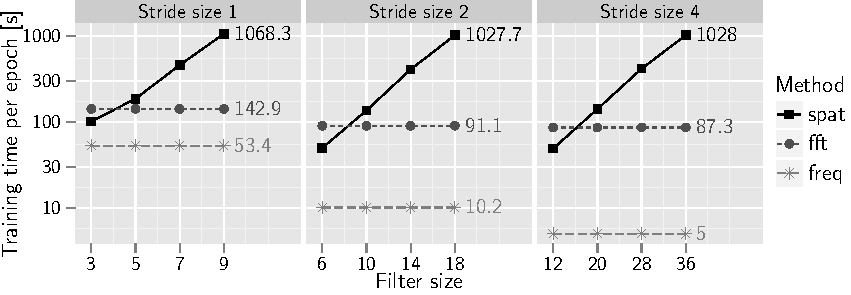
\includegraphics{figures/NECO-03-14-2099-Figure-4}
%\input{r_figures/runtime_oasis_c1_bw}
}

\subfloat[Running times of training a second layer sconvRBM with 8, 16, and 32
channels (stride size 1).] {
\label{fig:run_oasis_l2}
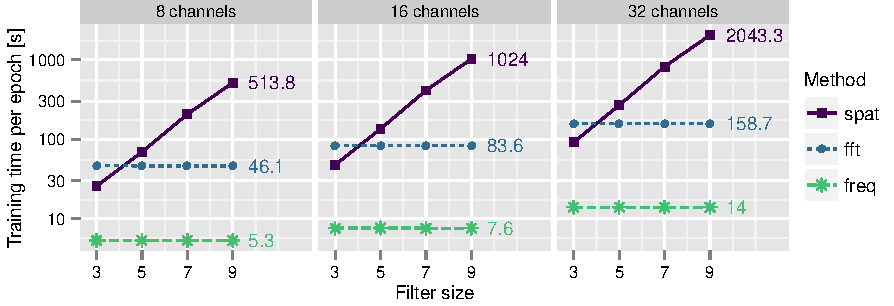
\includegraphics{figures/runtime_oasis_c8-32}
%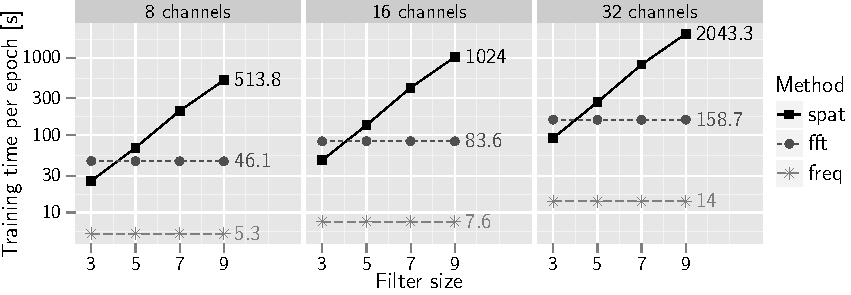
\includegraphics{figures/NECO-03-14-2099-Figure-5}
%\input{r_figures/runtime_oasis_c8-32_bw}
}
\caption[Comparison of running times for training a sconvRBMs on 3D
images]{Comparison of running times for training a (a) first and (b) second
layer sconvRBM on 3D volumes using a single 3D image convolution implementation
(spat), an implementation that calculates convolutions by using FFTs (fft), and
our proposed implementation in the frequency domain (freq).}
\label{fig:run_oasis}
\end{figure}

\subsection[Comparison of running times for calculating convolutions with
cuDNN]{Comparison of Running Times for Calculating Convolutions with cuDNN}

% TODO: Add used by Torch, Caffe, TensorFlow

The NVIDIA CUDA Deep Neural Network library (cuDNN) \citep{chetlur2014} is a
GPU-accelerated library of primitives that are frequently used to implement deep
learning methods such as CNNs and convDBNs. The library provides highly
optimized implementations for calculating, e.g., batched 2D and 3D convolutions,
pooling operations, and different transfer functions. In this set of
experiments, we directly compared the time required to calculate convolutions
when training a CNN using our frequency domain implementation with cuDNN. We
only consider convolutions because they are the most time-consuming operations
and because all other operations are calculating in the same way. For the
frequency domain implementation, all measurements include the time required to
calculate FFTs for calculating gradients and for transforming the accumulated
gradient to spatial domain in order to calculate the parameters updates. The
parameters that we used for evaluating the speed of different convolution
implementations are summarized in \ref{tab:cudnn_parameters}. The parameters
represent typical values of the first and second layer of a CNN, which are the
layers that typically take the most time to train. The key parameters that we
varied are the image size, filter size, and batch size. The hardware details of
our test environment are summarized in \ref{tab:cudnn_hardware}.

% TODO: explain training of CNNs: already have forward pass, but also need
% backwards pass and gradient calculation

% Experiments: - varying image size, batch size, filter size
%              - models used in this thesis (7-layer CEN, sconvDBN)
% Make this two subsubsections, one for detailed experiments and one for real
% models 
% Real models also show what reorganization does for you.
% Methods: frequency domain, frequency domain with padding, cuDNN
% Figure out what is common and what not.

\begin{table}
\centering
\caption{CNN layer parameters for the comparison with cuDNN.}
\label{tab:cudnn_parameters}
\begin{tabular}{cccccc}
\toprule
Experiment & \#Channels & Image size & Filter size & Filter count & Batch size
\\
\midrule
%\multirow{2}*{\minitab[c]{Varying\\ image size}} 
Varying & $2$  & $16^3, 17^3, \dotsc, 128^3$ & $9^3$ & $32$ & $8$ \\
image sizes & $32$ & $10^3, 11^3, \dotsc, 64^3$  & $9^3$ & $32$ & $8$ \\
\addlinespace
%\multirow{2}*{\minitab[c]{Varying\\ batch size}}
Varying & $2$  & $128^3$ & $9^3$ & $32$ & $1, 2, 4, 8$ \\
batch sizes & $32$ & $64^3$  & $9^3$ & $32$ & $1, 2, 4, 8$ \\
\addlinespace
%\multirow{2}*{\minitab[c]{Varying\\ filter size}}
Varying & $2$  & $128^3$ & $1^3, 2^3, \dotsc, 9^3$ & $32$ & $8$ \\
filter sizes & $32$ & $64^3$  & $1^3, 2^3, \dotsc, 9^3$ & $32$ & $8$ \\
\bottomrule
\end{tabular}
\end{table} 

\begin{table} 
\centering
\caption{Hardware specification of our test system for the comparison with
cuDNN.}
\label{tab:cudnn_hardware}
\begin{tabular} {ll}
\toprule
Processor & Intel i5-2500 CPU @ 3.30\,GHz \\
CPU Memory & 32\,GB \\
\addlinespace
Graphics Card & NVIDIA GeForce GTX 780 \\
GPU Cores & 2304 cores @ 0.94\,GHz \\
GPU Memory & 3\,GB \\
\bottomrule
\end{tabular}
\end{table}

\ref{fig:imagesize} shows a comparison of the running times for calculating
convolutions using our frequency domain implementation and cuDNN for varying
image sizes. The FFT implementation that we used internally, cuFFT, is optimized
for image sizes that can be factorized as $2^a\times3^b\times5^c$. Therefore, we
also evaluated the time required to calculate convolutions when the input images
are automatically padded to a size for which cuFFT has been optimized. For image
sizes larger than $110^3$ voxels, cuFFT requires significantly more temporary
memory for calculating FFTs of unoptimized image sizes. Consequently, only the
running times of the padded frequency domain implementation and cuDNN were
measured for image sizes larger than $110^3$ voxels. Calculating convolutions in
the frequency domain scale better with increasing image size than cuDNN. While
cuDNN is the fastest method for very small image sizes, the padded frequency
domain implementation is more than 20 times faster for images with a size of
$128^3$ voxels and 2 input channels, and more than 18 times faster for images
with a size of $64^3$ voxels and 32 channels. Calculating the FFT and therefore
the running time of the frequency domain implementation varies significantly
depending on the input image size, and careful padding of the input images is
required to achieve consistently high performance.

% \begin{itemize}
% \item Improvements over cuDNN are larger for higher number of channels where the
% impact of calculating the FFT on the overall running time is also lower
% \item Going from 2 to 32 channels, the observed speed-up increases from
% approximately 10 times for the 2 channel comparison to approximately 18 times
% for the 32 channel comparison.
% \item Although the non-padded frequency domain implementation varies less for 32
% channels than for the 2 channel case, padding is still advantageous.
% \end{itemize}

\begin{figure}
\centering
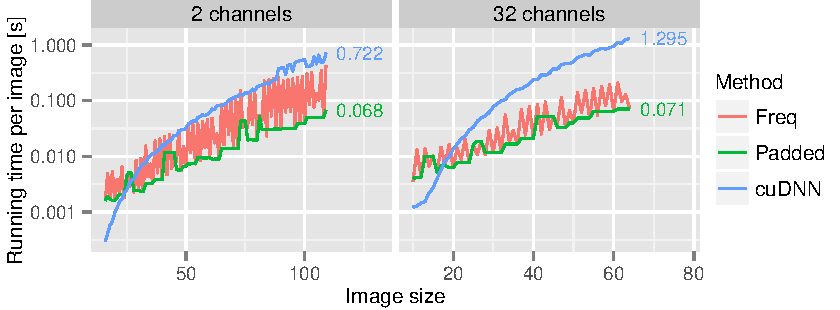
\includegraphics[width=0.95\textwidth]{figures/imagesize}
\caption[Comparison of running times of key operations for training a single
CNN layer.]{Comparison of running times of key operations for training a single
CNN layer for varying number of channels and input sizes. Frequency domain
training and training using cuDNN scales comparable for small numbers of
channels. For large numbers of channels, frequency domain method scales
slightly better to larger images.}
\label{fig:imagesize}
\end{figure}

\ref{tab:batchsize} shows a comparison of running times per image for varying
batch sizes and for varying number of channels. Increasing the batch size has
only a minor effect on the running time of cuDNN, while significantly increasing
the required amount of GPU memory. In contrast, the implementation in the
frequency domain does not require more memory, because each image of a
mini-batch is processed sequentially. Increasing the batch size reduces the
average running time per image of our frequency domain implementation, because
the FFTs required to calculate the parameter updates need to be calculated only
once per mini-batch, and have therefore a smaller impact on the overall running
time when the number of images per mini-batch is larger.

\begin{table}[tb]
\centering
\caption[Comparison of running times for calculating key operations for training
a CNN layer for different batch sizes]{Comparison of running times for
calculating key operations for training a CNN layer for different batch sizes.
Increasing the batch size reduces the impact of cropping the learned filters on
the overall running time and consequently reduces the average time to process
one image. The cuDNN implementation only benefits mildly from using larger
batches.}
\label{tab:batchsize}

\sisetup{
  round-mode = places,
  round-precision = 3,
  exponent-product = \cdot,
  detect-weight=true,
  detect-inline-weight=math,
  tight-spacing = false,
  table-align-text-post = false
}%
\begin{tabular}{
S[table-format=2.0]
S[table-format=1.3]
S[table-format=1.3]
S[table-format=1.3]
S[table-format=1.3]
S[table-format=1.3]
}
\toprule
{Batch size} & \multicolumn{4}{c}{Running time [s]} \\ 
& \multicolumn{2}{c}{$2$ channels} & \multicolumn{2}{c}{$32$
channels}
\\
           & {Freq} & {cuDNN} & {Freq} & {cuDNN} \\
\midrule
1   &  0.108588  & 1.39723 & 0.152864 & 1.31284 \\
2   &  0.0814377 & 1.01137 & 0.105898 & 1.30724 \\
4   &  0.0679075 & 1.24905 & 0.082375 & 1.30408 \\
8   &  0.0603056 & 1.24731 & 0.070710 & 1.29555 \\
%16  &  0.0568994 & {---}     & 0.064798 & 1.29431 \\
\bottomrule
\end{tabular}
\end{table}

The impact of the filter size on running time is shown in \ref{fig:filtersize}.
Training in the frequency domain is faster for all filter sizes, where the
speed-ups are larger for larger filters. At a filter size of $9$, the speed-up
is 20 times. For $32$ channels, cuDNN is faster for very small filter sizes and
training in the frequency domain breaks even at a filter size of $3$.
For filter sizes larger than $3$, training in the frequency domain is
substantially faster with a speed-up of up to $18$ times a filter size of $9$.

\begin{figure}
\centering
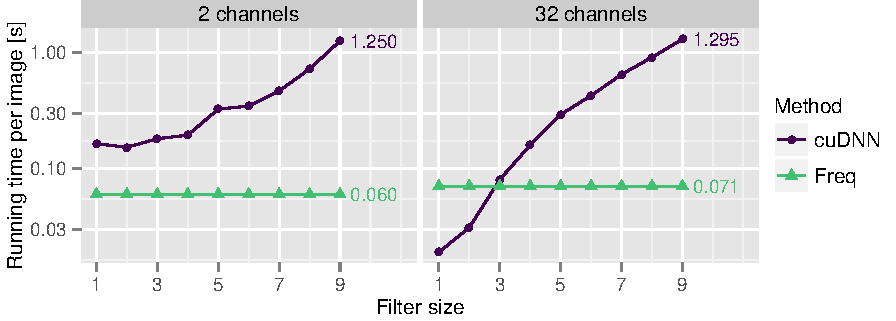
\includegraphics[width=0.9\textwidth]{figures/filtersize}
\caption[Comparison of running times of key operations for training a single
CNN layer.]{Comparison of running times of key operations for training a single
CNN layer for varying number of channels and filter sizes.}
\label{fig:filtersize}
\end{figure}

\ref{tab:usedmodels} shows a comparison of running times for calculating
convolutions of our frequency domain implementation with cuDNN for the 7-layer
convolutional encoder network (CEN) that is used in \ref{sec:segmentation} to
segment MS lesions, and the first sconvRBM of the DBN model described in
\ref{sec:manifold} to model the variability in lesion distribution and brain
morphology. For the 7-layer CEN, the second convolutional and the first
deconvolutional layer benefits the most from training in the frequency domain
due to the relatively large number of channels in these layers. Overall, the
convolutions required to train the 7-layer CEN can be calculated 6.3 times
faster in the frequency domain compared to cuDNN. In a second experiment, we
compared the time required to directly calculate strided convolutions with
mapping strided convolutions to stride-1 convolutions by reorganizing the
visible units of an sconvRBM. For the frequency domain implementation, the
direct method calculates stride-1 convolutions instead of strided
convolutions and discards the unnecessary hidden units afterwards, because
strided convolutions cannot directly be calculated in the frequency domain.
Mapping strided convolutions to stride-1 convolutions speeds up the training in
the frequency domain by a factor of four compared to calculating stride-1
convolutions in the frequency domain. Overall, calculating the convolutions for
training the first sconvRBM is 3.7 times faster using our frequency domain
implementation than the direct implementation of strided convolutions of cuDNN.

\begin{table}
\caption[Comparison of running times of time critical operations of two example
deep learning models.]{Comparison of running times of time critical operations
of the 7-layer CEN-s used for segmentating lesions, and the first sconvRBM of
the lesion DBN using to model lesion distribution. The running times of pooling
layers we excluded.}
\label{tab:usedmodels}
\centering
\sisetup{
  round-mode = places,
  round-precision = 3,
  exponent-product = \cdot,
  detect-weight=true,
  detect-inline-weight=math,
  tight-spacing = false,
  table-align-text-post = false
}%

\begin{tabular}{l>{\raggedright}p{5cm}S[table-format=1.3]S[table-format=1.3]@{}S[table-format=2.3]}
\toprule
\multicolumn{2}{c}{Experiment} & \multicolumn{2}{c}{Running time
[s]\phantom{he}} & {Speed-up}
\\
& & {Freq} & {cuDNN} &  \\
\midrule
\multirow{5}*{\minitab[l]{$7$-layer CEN\\ used for lesion\\ segmentation}}
& 1st convolutional layer & 0.076582 & 0.498335 & 6.5072 \\
& 2nd convolutional layer & 0.0519153 & 0.523849 & 10.0904 \\
& 1st deconvolutional layer & 0.0519153 & 0.523849 & 10.0904 \\
& 2nd deconvolutional layer & 0.1477196 & 0.51716 & 3.500957 \\[0.5em]
& total & 0.3281322 & 2.063193 & 6.28768831587 \\
\midrule
\multirow{4}*{\minitab[l]{First sconvRBM of \\ the lesion DBN}}
& direct calculation of strided convolutions & 0.0755562 & 0.0683263 &
0.90431096323 \\
& strided convolutions mapped to stride-1 convolutions & 0.0186432 & 0.0705788 &
3.78576639204 \\
\bottomrule
\end{tabular}
\end{table}

\section{Conclusions}

We have presented a fast training method for convolutional models, which
performs training in the frequency domain in order to replace the time-consuming
computation of convolutions with simple element-wise multiplications. We have
shown that it is also essential to map the other operations to frequency space
wherever possible to minimize the number of Fourier transforms, and that this
greatly decreases training times over performing only the convolutions in the
frequency domain. In addition, our method can be efficiently implemented on the
GPU and is faster than a highly optimized GPU implementation of batched
convolutions in the spatial domain. We have evaluated the running time
improvements using two standard benchmark datasets, showing a speed-up of up to
8 times on 2D images from the ImageNet dataset and up to 200 times on 3D volumes
from the OASIS dataset. In addition, we have directly compared to the time
required to calculate convolutions using our method with cuDNN, the current
state-of-the-art library for calculating 2D and 3D convolutions, with the
results showing that our method can calculate convolutions up to 20 times faster
than cuDNN.

% TODO: emphasize the key features compared to other FD implementations
% Only efficient when flipping can be expressed in the frequency domain
% otherwise either store flipped and non-flipped versions, which increases
% the amount of required memory, or requires flipped in spatial domain, which
% adds FFT calculations, or do it in batch-mode, which also increases memory
